\documentclass[11pt]{article}

% Generated by tools/author/maptex.py. Do not edit; edit the map's author script
% and run it again.

\usepackage[T1]{fontenc}
\usepackage[utf8]{inputenc}
\usepackage[margin=0.85in]{geometry}
\usepackage{amsmath}
\usepackage{kpfonts}
\usepackage{tikz}
\usetikzlibrary{arrows.meta}
\usepackage{enumitem}
\usepackage{multicol}
\usepackage{xcolor}
\usepackage{url}

\definecolor{maroon}{HTML}{800000}
\definecolor{inkgrey}{HTML}{4D4D4D}

% An explicit white page. Without it the page background is undefined, and a viewer
% or a converter that composites onto black renders the body text invisible.
\pagecolor{white}

\pagestyle{empty}
\setlength{\parindent}{0pt}
\setlength{\parskip}{0.6em}

\newcommand{\heading}[1]{%
  \par\medskip{\large\bfseries\color{maroon} #1}\par\smallskip}

\tikzset{
  concept/.style={rectangle, draw=inkgrey, rounded corners=2pt,
    align=center, font=\footnotesize, inner sep=3pt, fill=white, line width=0.5pt},
  edgenum/.style={circle, fill=white, draw=inkgrey, inner sep=0pt,
    minimum size=11pt, font=\scriptsize\bfseries, line width=0.4pt},
  nlabel/.style={font=\tiny\bfseries, text=inkgrey, inner sep=1pt},
  % One arrow style, on the worksheet and on the key alike. Nothing is withheld any
  % more, so the head is drawn, and a relationship that runs both ways gets two of
  % them. No hyphens in these names: tikz reads a hyphen as an arrow-tip spec.
  kindholds/.style={-{Latex[length=2mm]}, thick, inkgrey},
  kindequiv/.style={{Latex[length=2mm]}-{Latex[length=2mm]}, thick, inkgrey},
}

\begin{document}

{\LARGE\bfseries\color{maroon} Infinite series}\par\medskip
{\color{inkgrey}\small Math 163 \quad\textbullet\quad Prof.\ Chowdhury}\par\bigskip

The next page has 15 ideas as boxes, with 16 numbered arrows between them and nothing written on any arrow. Each arrow is a relationship that holds in the direction drawn. Some are implications between properties. Some record that one box is defined in terms of another. Many name the theorem that decides a question about the box the arrow points at: the integral test applied to \(1/x^p\) determines exactly which exponents make \(\sum 1/n^p\) converge.

For each numbered arrow, state the relationship in one sentence. Name the theorem where there is one, and give the hypothesis it turns on. An arrow with a head at each end holds in both directions.

When you have had a go at all of them, check yourself at \url{subhadipchowdhury.github.io/teaching/labs/maps/series/}. That page draws the same map and will show you the answers one arrow at a time, or all at once.

\heading{What each box means}
\small
\begin{enumerate}[label=\textbf{\Alph*.}, leftmargin=2.2em, itemsep=1pt]
\item \textbf{Infinite Series \(\sum a_n\).} The expression \(a_1 + a_2 + a_3 + \cdots\). It has no meaning until the partial sums give it one.
\item \textbf{Partial Sums \(\{s_n\}\).} \(s_n = a_1 + \cdots + a_n\). An ordinary sequence, so everything you know about sequences applies to it.
\item \textbf{Convergent Series.} \(\sum a_n\) converges when \(\{s_n\}\) has a finite limit, and the sum is that limit.
\item \textbf{Divergent Series.} \(\sum a_n\) diverges when \(\{s_n\}\) fails to converge, whether it runs away or oscillates.
\item \textbf{Divergence Test.} If \(a_n \not\to 0\) then \(\sum a_n\) diverges. It is a test for divergence only, and it never certifies convergence.
\item \textbf{Geometric Series.} \(\sum ar^n\), which converges exactly when \(|r| < 1\), with sum \(a/(1-r)\) and partial sums \(a(1-r^n)/(1-r)\).
\item \textbf{Telescoping Series.} \(\sum (b_n - b_{n+1})\), whose partial sums collapse to \(b_1 - b_{n+1}\).
\item \textbf{\(p\)-Series \(\sum 1/n^p\).} Converges exactly when \(p > 1\). The boundary \(p = 1\) is the harmonic series, which diverges.
\item \textbf{Nonneg Series \(+\) MCT.} If \(a_n \ge 0\) the partial sums increase, so the monotone convergence theorem turns convergence into boundedness.
\item \textbf{Comparison Tests.} Direct: \(0 \le a_n \le cb_n\) eventually and \(\sum b_n\) convergent gives \(\sum a_n\) convergent. Limit: \(\lim a_n/b_n \in (0,\infty)\) gives the same behaviour for both.
\item \textbf{Integral Test.} If \(f\) is positive, continuous and eventually decreasing with \(f(n) = a_n\), then \(\sum a_n\) and \(\int_1^\infty f\) converge or diverge together.
\item \textbf{Dirichlet's Test.} If \(a_n\) decreases to \(0\) and the partial sums of \(b_n\) are bounded, then \(\sum a_n b_n\) converges. Proved by summation by parts.
\item \textbf{Absolute Convergence.} \(\sum a_n\) converges absolutely when \(\sum |a_n|\) converges. This is strictly stronger than convergence.
\item \textbf{Conditional Convergence.} \(\sum a_n\) converges conditionally when it converges and \(\sum |a_n|\) does not. The convergence rests on cancellation.
\item \textbf{Ratio and Root Tests.} With \(L = \lim |a_{n+1}/a_n|\) or \(L = \limsup |a_n|^{1/n}\): absolutely convergent if \(L < 1\), divergent if \(L > 1\), and no conclusion if \(L = 1\).
\end{enumerate}
\normalsize
\newpage
\vspace*{\fill}
\begin{center}
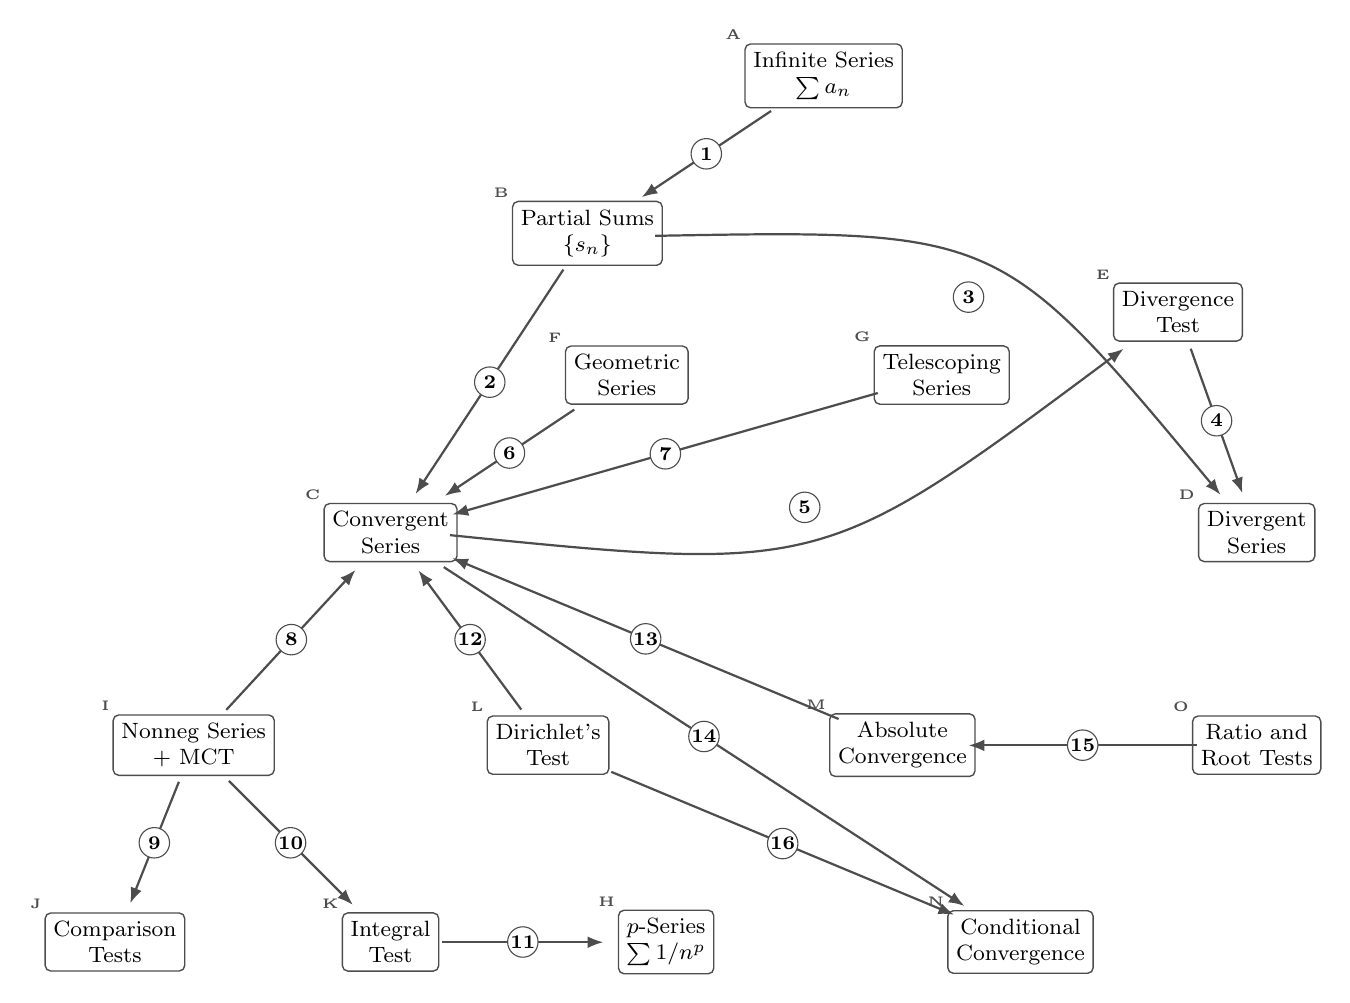
\begin{tikzpicture}[>=Latex]
  \node[concept] (A) at (1.5, 0) {Infinite Series \\ \(\sum a_n\)};
  \node[concept] (B) at (-1.5, -2) {Partial Sums \\ \(\{s_n\}\)};
  \node[concept] (C) at (-4, -5.8) {Convergent \\ Series};
  \node[concept] (D) at (7, -5.8) {Divergent \\ Series};
  \node[concept] (E) at (6, -3) {Divergence \\ Test};
  \node[concept] (F) at (-1, -3.8) {Geometric \\ Series};
  \node[concept] (G) at (3, -3.8) {Telescoping \\ Series};
  \node[concept] (H) at (-0.5, -11) {\(p\)-Series \\ \(\sum 1/n^p\)};
  \node[concept] (I) at (-6.5, -8.5) {Nonneg Series \\ \(+\) MCT};
  \node[concept] (J) at (-7.5, -11) {Comparison \\ Tests};
  \node[concept] (K) at (-4, -11) {Integral \\ Test};
  \node[concept] (L) at (-2, -8.5) {Dirichlet's \\ Test};
  \node[concept] (M) at (2.5, -8.5) {Absolute \\ Convergence};
  \node[concept] (N) at (4, -11) {Conditional \\ Convergence};
  \node[concept] (O) at (7, -8.5) {Ratio and \\ Root Tests};

  \node[nlabel, anchor=south east] at (A.north west) {A};
  \node[nlabel, anchor=south east] at (B.north west) {B};
  \node[nlabel, anchor=south east] at (C.north west) {C};
  \node[nlabel, anchor=south east] at (D.north west) {D};
  \node[nlabel, anchor=south east] at (E.north west) {E};
  \node[nlabel, anchor=south east] at (F.north west) {F};
  \node[nlabel, anchor=south east] at (G.north west) {G};
  \node[nlabel, anchor=south east] at (H.north west) {H};
  \node[nlabel, anchor=south east] at (I.north west) {I};
  \node[nlabel, anchor=south east] at (J.north west) {J};
  \node[nlabel, anchor=south east] at (K.north west) {K};
  \node[nlabel, anchor=south east] at (L.north west) {L};
  \node[nlabel, anchor=south east] at (M.north west) {M};
  \node[nlabel, anchor=south east] at (N.north west) {N};
  \node[nlabel, anchor=south east] at (O.north west) {O};

  \draw[kindholds] (0.833, -0.446) .. controls (0.011, -0.994) .. (-0.811, -1.542);
  \draw[kindholds] (-1.805, -2.46) .. controls (-2.744, -3.886) .. (-3.683, -5.311);
  \draw[kindholds] (-0.641, -2.032) .. controls (3.739, -1.952) .. (6.54, -5.321);
  \draw[kindholds] (6.162, -3.466) .. controls (6.491, -4.384) .. (6.819, -5.302);
  \draw[kindholds] (-3.245, -5.833) .. controls (1.493, -6.311) .. (5.311, -3.465);
  \draw[kindholds] (-1.667, -4.239) .. controls (-2.489, -4.787) .. (-3.311, -5.335);
  \draw[kindholds] (2.188, -4.028) .. controls (-0.513, -4.799) .. (-3.214, -5.571);
  \draw[kindholds] (-6.086, -8.052) .. controls (-5.265, -7.163) .. (-4.444, -6.274);
  \draw[kindholds] (-6.688, -8.965) .. controls (-6.997, -9.737) .. (-7.306, -10.51);
  \draw[kindholds] (-6.053, -8.954) .. controls (-5.266, -9.741) .. (-4.478, -10.529);
  \draw[kindholds] (-3.348, -11.003) .. controls (-2.322, -11.003) .. (-1.297, -11.003);
  \draw[kindholds] (-2.34, -8.048) .. controls (-2.993, -7.164) .. (-3.646, -6.28);
  \draw[kindholds] (1.69, -8.168) .. controls (-0.763, -7.146) .. (-3.217, -6.124);
  \draw[kindholds] (-3.324, -6.239) .. controls (-0.018, -8.391) .. (3.289, -10.543);
  \draw[kindholds] (6.238, -8.503) .. controls (4.79, -8.503) .. (3.341, -8.503);
  \draw[kindholds] (-1.197, -8.839) .. controls (0.981, -9.747) .. (3.158, -10.654);

  \node[edgenum] at (0.01, -0.99) {1};
  \node[edgenum] at (-2.74, -3.89) {2};
  \node[edgenum] at (3.34, -2.81) {3};
  \node[edgenum] at (6.49, -4.38) {4};
  \node[edgenum] at (1.26, -5.48) {5};
  \node[edgenum] at (-2.49, -4.79) {6};
  \node[edgenum] at (-0.51, -4.80) {7};
  \node[edgenum] at (-5.26, -7.16) {8};
  \node[edgenum] at (-7.00, -9.74) {9};
  \node[edgenum] at (-5.27, -9.74) {10};
  \node[edgenum] at (-2.32, -11.00) {11};
  \node[edgenum] at (-2.99, -7.16) {12};
  \node[edgenum] at (-0.76, -7.15) {13};
  \node[edgenum] at (-0.02, -8.39) {14};
  \node[edgenum] at (4.79, -8.50) {15};
  \node[edgenum] at (0.98, -9.75) {16};
\end{tikzpicture}
\end{center}
\vspace*{\fill}
\newpage
\heading{The arrows}
\small
\begin{multicols}{2}
\begin{enumerate}[label=\textbf{\arabic*.}, itemsep=0.7em, leftmargin=1.8em]
\item
  \dotfill\\[3pt]\dotfill
\item
  \dotfill\\[3pt]\dotfill
\item
  \dotfill\\[3pt]\dotfill
\item
  \dotfill\\[3pt]\dotfill
\item
  \dotfill\\[3pt]\dotfill
\item
  \dotfill\\[3pt]\dotfill
\item
  \dotfill\\[3pt]\dotfill
\item
  \dotfill\\[3pt]\dotfill
\item
  \dotfill\\[3pt]\dotfill
\item
  \dotfill\\[3pt]\dotfill
\item
  \dotfill\\[3pt]\dotfill
\item
  \dotfill\\[3pt]\dotfill
\item
  \dotfill\\[3pt]\dotfill
\item
  \dotfill\\[3pt]\dotfill
\item
  \dotfill\\[3pt]\dotfill
\item
  \dotfill\\[3pt]\dotfill
\end{enumerate}
\end{multicols}
\normalsize
\heading{Counterexamples and benchmarks}
\small
\begin{itemize}[leftmargin=1.4em, itemsep=1pt]
\item The harmonic series \(\sum 1/n\) diverges even though its terms tend to zero.
\item The alternating harmonic series \(\sum (-1)^{n+1}/n\) converges conditionally, to \(\ln 2\).
\item \(\sum \sin(n\theta)/n\) converges by Dirichlet's test and is not alternating.
\item Summation by parts is the discrete integration by parts, and it is what proves Dirichlet's test.
\item The Cauchy criterion for series: control every far enough tail at once, not one chosen tail.
\end{itemize}
\normalsize
\heading{One last question}
Which single arrow carries the most of this chapter? There is more than one defensible answer, and the argument is the useful part.
\par\medskip\dotfill\\[4pt]\dotfill\\[4pt]\dotfill

\vfill
{\scriptsize\color{inkgrey} Contents by Subhadip Chowdhury, licensed CC BY-NC-SA 4.0. Built with AI assistance. I checked the mathematics myself.\par}
\end{document}
